\documentclass{beamer}
\usepackage{graphicx}
\usepackage{wrapfig}
\usepackage{setspace}
\usepackage{xcolor}
\usetheme{Madrid}
\usecolortheme{default}

\title[2020MP000]{Video Streaming Platform for open source community}
\subtitle{Project ID:21C131176\\Review -II}
\author[SRM Institute of Science \& Technology]{Group~Members\\RA1711003030131~Kanishk Dixit \\RA1711003030176~Akshay Jain\\ \medskip{Supervised By:\\Mr. Abhishek Singh \\Assistant Professor}}
\institute[]{Department of Computer Science \& Engineering\\Faculty of Engineering \& Technology\\SRM Institute of Science \& Technology}
\logo{\includegraphics[scale=.4]{srm_logo}}
%\author{YYY}
\date{\today}
\begin{document}
	\begin{frame}
		\maketitle
		\date{}
	\end{frame}
	\begin{frame}[t]{Table of Contents} %we can expand the table of contents in more than on frame
		\tableofcontents[sections={1-6}]
	\end{frame}
	\section{Objective}
	\begin{frame}{Objective}
\begin{itemize}
    \item To provide the video streaming experience in a better way over the internet.
    \item To provide a platform for content creators to market there content to the specified users.

    \item  To provide easy accessibility of a specific content to the content consumers.
    \item Create an open source community for this platform.

\end{itemize}	  
	\end{frame}
	\section{Literature Survey}
	\begin{frame}[allowframebreaks]{Literature Survey}
	\begin{itemize}
		
		\item   \textbf{Speech Recognition using Recurrent  Neural Networks} \\
		\textbf{Authors-:} \textbf{Aditya Amberkar},\textbf{Parikshit Awasarmol} MCT’s Rajiv Gandhi Institute of Technology, Mumbai, Maharashtra. \\
			\vspace{0.5cm}
		\textbf{Description:} RNN is one of the best algorithm used for processing of speech  signal  and  it  has  scope  in  emerging  voice controlled  technologies  but  training  algorithm  is  again needed. \\
		\vspace{0.5cm}
		It  shows  better  results  than  Multilayer perceptron(MLP).Speech  recognition  has  attracted many scientists and researchers and can be influential to society in  emerging  technologies.  This  paper  give  basic understanding  of  Speech  Processing  using  Recurrent Network and various STT Engine available which can be used for application development
		
		\item \textbf{Convolutional Neural Networks for Raw Speech Recognition}\\
		\textbf{Author-:Vishal Passricha and Rajesh Kumar Aggarwal}\\
		\vspace{0.5cm}
		\textbf{Description-:}This paper discusses the CNN-based direct raw speech recognition model. This model directly learns the relevant representation from the speech signal in a data-driven manner and calculates the conditional probability for each phoneme class. In this, CNN as an acoustic model consists of a feature stage and classifier stage. Both the stages are trained jointly. Raw speech is supplied as input to first convolutional layer, and it is further processed by several convolutional layers. Classifiers like ANN, CRF, MLP, or fully connected layers calculate the conditional probabilities for each phoneme class. After that decoding is performed using HMM. This model shows the similar performance as shown by MFCC-based conventional mode.
		\item \textbf{A study on automatic speech recogntion}\\
		\vspace{0.5 cm}
		\textbf{Authors:-Sai Benk , Yussuf Elimmir}\\
		\textbf{Description-}Previous studies have tried to focus on the major gaps in the Automatic Speech Recognition System and identified solutions that reduce those gaps and the percentage of errors. This research examined all the phases of the automatic speech recognition systems (Acoustic pre-processing, pronunciation model, acoustic model, language model) but also agreed on a common objective: use of neural networks;  when they used the HMM/DNN hybrid model. All these studies have validated the use of neural networks to get better results both with other techniques or without them and this is what is observed in all the results of this work, also the use of this type of networks brings several advantages to the field of automatic speech processing.
		
		\end{itemize} 
	\end{frame}
\section{Architectural Design For Proposed System}
\begin{frame}[allowframebreaks]{Architectural Design For Proposed System}
    \begin{figure}
		{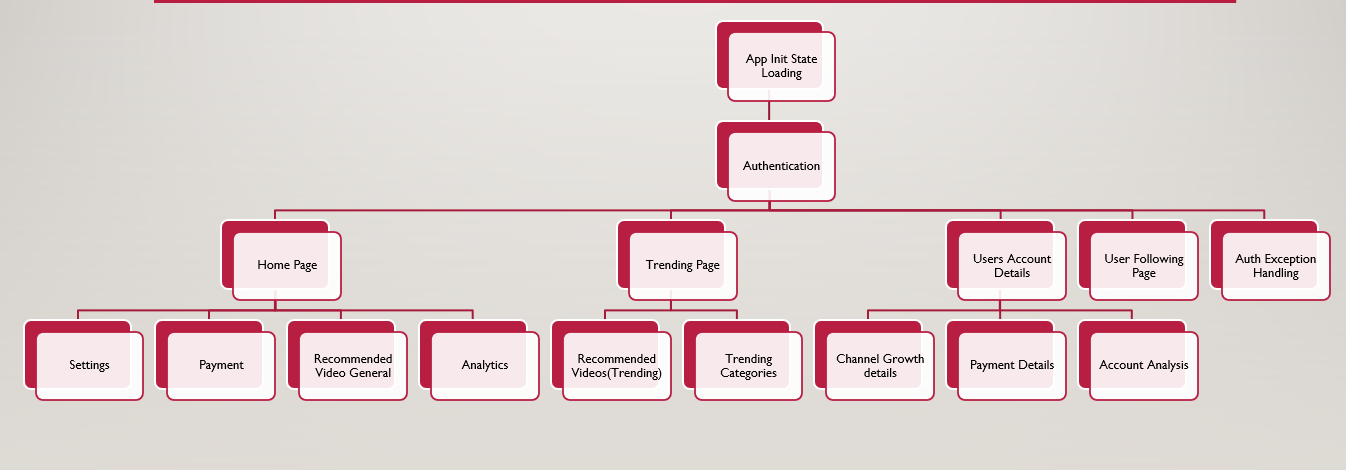
\includegraphics[scale=.4]{arch.PNG}}
			\caption{Proposed Architecture}
			\label{arch1}
	\end{figure}
	\begin{center}
	\textcolor{red}{\textit{Explanation of project Architecture: }}\\
	\begin{itemize}
		\item  System Would Accept input in the form of speech from the user 
		\item  Once the user has provided the speech input, the system would recognise the words in the speech using the python speechrecognition module and provide text output.
		\item  once the text is obtained, the program would analyse the text for various keywords and call the respective modules. 
		\item  Based on the module called, the program will continue and provide the required output in form of speech.
		\end{itemize}
    \end{center}
\end{frame}
\section{Proposed Software Design}
\begin{frame}[allowframebreaks]{Proposed Software Design}
    \begin{figure}
		{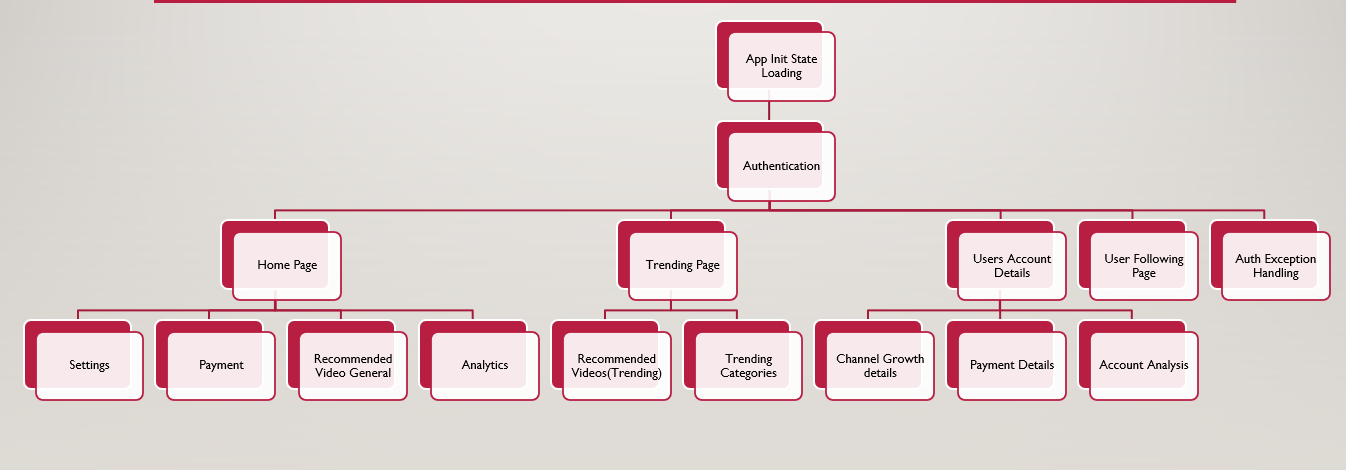
\includegraphics[scale=.4]{arch.PNG}}
			\caption{Proposed Design}
			\label{arch}
	\end{figure}
	\begin{center}
	\textcolor{red}{\textit{Explanation of Software Design: }}\\
	\begin{itemize}
		\item  On Launching the software, the user will be greeted by a main GUI screen that will have buttons to launch all the indivisual modules and a common mic button that will accept speech input and detect keywords to launch the modules.
		\item  Indivisual GUI buttons will be made for Translator, Weather Forecast, Game, Main Mic and emotion detection.
		\item  Based on the button clicked or keyword detected modules will be launched.
		\item  After the execution of the module speech output will be given.
		\end{itemize}
    \end{center}
	
\end{frame}
\section{Techniques to be used}
\begin{frame}[t]{Techniques to be used}
    \begin{center}
	\LARGE
	\textcolor{red}{\textit{Project is Divided into various parts that are executed as follows : }}\\ 
    \end{center}
	\begin{itemize}
		\item Speech Recognition : Executed by using speechrecognizer header file of python that converts speech to text. the text is then used to carry out various operations.
		\item Speech Output : To execute this part we have utilized python-text-to-speech engine(pyttsx3) which takes text input and provides speech output. 
		\item  Emotion Recognition : To detect the emotions in the words of the user's speech we utilize the textblob module of python which provides the neutrality of the text.
		\item Weather Forecasting : The software is able to provide the weather details in a particular area which is achieved by using openweathermap API. 
	\end{itemize}
	\end{frame}
\section{References}
\begin{frame}[t]{References}
    \begin{center}
        \begin{itemize}
            \vspace{1 cm}
            \item Speech Recognition using Recurrent Neural NetworksAuthors-: Aditya Amberkar,Parikshit AwasarmolMCT’s RajivGandhi Institute of Technology, Mumbai, Maharashtra.
            \vspace{1 cm}
            \item Convolutional Neural Networks for Raw Speech RecognitionAuthor-:Vishal Passricha and Rajesh Kumar Aggarwal
        \end{itemize}
    \end{center}
\end{frame}


\end{document}